\documentclass[11pt]{article}
\usepackage[margin=0.7in]{geometry}
\usepackage{multirow}
\usepackage {graphicx}
\usepackage[utf8x]{inputenc} % указать кодировку русского текста
\usepackage[russian]{babel} % указать, что язык текста - русский
\usepackage{fancyhdr}
\pagestyle{fancy}

\begin{document}

\begin{titlepage}

\begin{center}
%\vspace*{1cm}
\large\textbf{Московский Физико-Технический Институт}\\
\large\textbf{(государственный университет)}
\vfill
\line(1,0){430}\\[1mm]
\huge\textbf{Релаксационные колебания}\\
\line(1,0){430}\\[1mm]
\vfill
\large Сибгатуллин Булат, ФРКТ\\
\end{center}

\end{titlepage}
\fancyhead[L] {Работа 2.3.1}
\noindent \textbf{Цель работы:} \\
\indent изучение вольт-амперной характеристики нормального тлеющего разряда; исследование релаксационного генератора на стабилитроне.\\
\noindent \textbf{В работе используются:} \\
\indent стабилитрон СГ-2 (газонаполненный диод) на монтажной панели, амперметр, магазин сопротивлений, магазин ёмкостей, источник питания, осциллограф (ЭО), генератор звуковой частоты (ЗГ).
\section*{Описание работы}\

Зависимость тока от напряжения для газоразрядной лампы не подчиняется закону Ома и характеризуется рядом особенностей, ее вольтамперная характеристика указана на рис. 1.

\begin{figure}[h!]
\centering
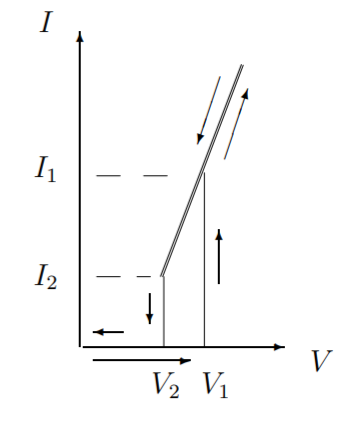
\includegraphics[scale=0.8]{Image1.png}
\label{fig:Image1}
\caption{Вольтамперная характеристика стабилитрона с последовательно включенным резистором}
\end{figure}

При малых напряжениях лампа практически не пропускает ток. Как только разность потенциалов на ее электродах достигает напряжения зажигания в лампе начинает течь ток. После, так как наш источник напряжения не может поддерживать такую силу тока, напряжение на лампе начинает падать и достигая напряжения гашения, силу тока на ней скачком падает до нуля.

\begin{figure}[h!]
\centering
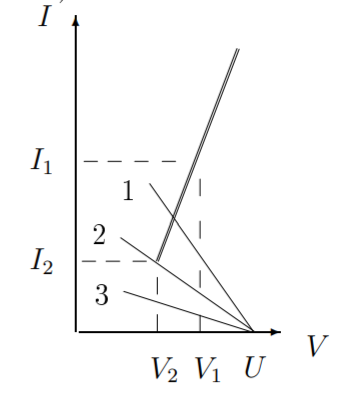
\includegraphics[scale=0.8]{Image3.png}
\label{fig:Image1}
\caption{Режимы работы релаксационного генератора}
\end{figure}

Колебательный процесс возможен когда нагрузочная прямая не пересекает характеристику лампы (3 прямая на рис. 3). Это происходит из-за того, что в стационарном режиме ток черещ лампу равен:

\[I_{\textit{ст}} = \frac{U - V}{R},\]

где $V$ - напряжение на конденсаторе и оно постоянно. Тогда прямая 2 проходящая через точку $(I_2, V_2)$, соответствует критическому сопротивлению:

\[R_{\textit{кр}} = \frac{U - V_2}{I_2},\]

тогда для $R > R_{\textit{кр}}$ в системе установятся колебания.

\begin{figure}[h!]
\centering
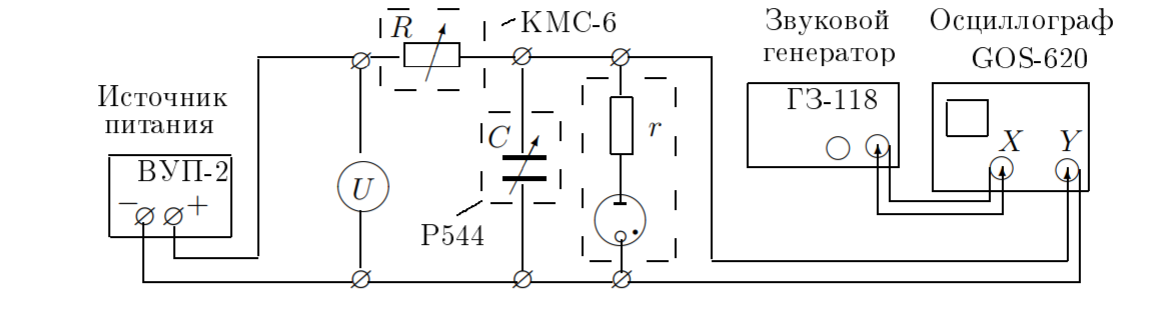
\includegraphics[scale=0.8]{Image2.png}
\label{fig:Image1}
\caption{Схема установки для изучения релаксационных колебаний}
\end{figure}

Схема установки изображена на рис. 3. Здесь период колебаний будет складываться из времени заряда $\tau_{\textit{з}}$ и времения разряда $\tau_{\textit{р}}$. В случае, когда сопротивление $R$ существенно превосходит внутреннее сопротивление стабилитрона, справедливо соотношение $\tau_{\textit{з}} \gg \tau_{\textit{р}}$. В таком случае период колебаний можно посчитать при помощи такой формулы:

\begin{equation}
T \approx \tau_{\textit{з}} = RC\ln \frac{U - V_2}{U - V_1},
\end{equation}

где $V_1$ и $V_2$ потенциалы зажигания и гашения соответственно.

\newpage

\section*{Ход работы}\

Снимем вольтамперную характеристику стабилитрона, внутреннее сопротивление стабилитрона $r = 5,1$ \textit{кОм}. Запишем данные в таблицу для систем из стабилитрона и дополнительного сопротивления \textit{r} и для стабилитрона без сопротивления \textit{r}. Построим графики зависимости $I = f(V)$ по данным таблицам.

\begin{figure}[h!]
\centering
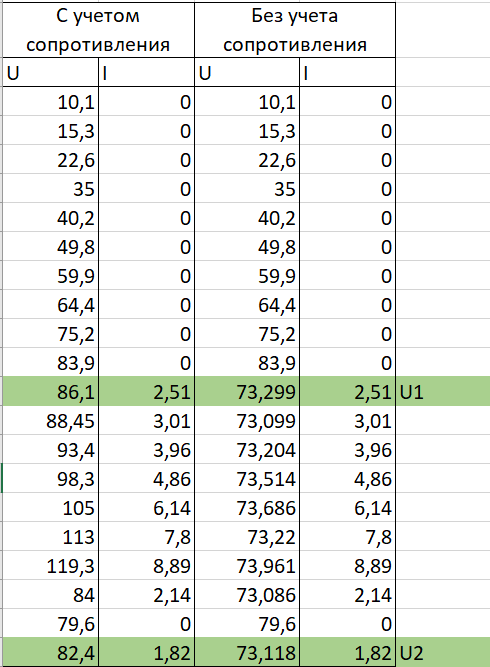
\includegraphics[scale=1]{table1.png}
\label{fig:Image1}
\caption{Зависимость U(I)}
\end{figure}

\begin{figure}[h!]
\centering
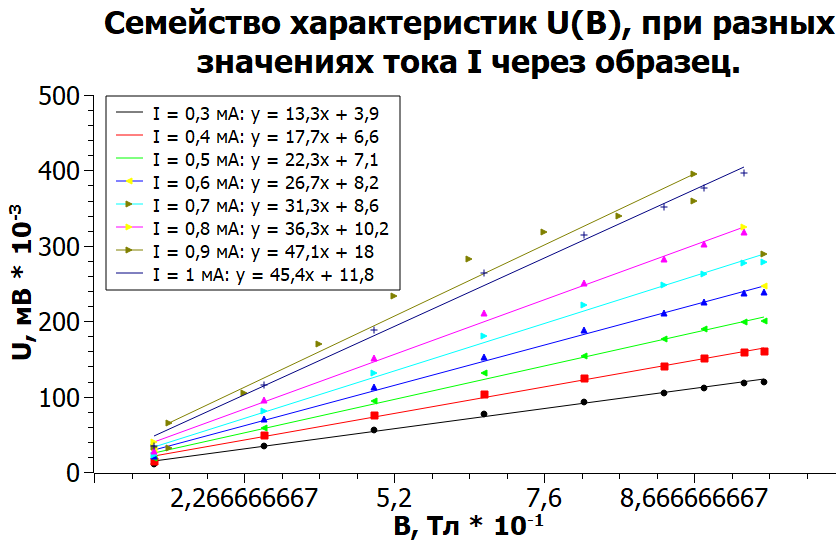
\includegraphics[scale=1]{Graph1.png}
\label{fig:Image1}
\end{figure}

\vspace{0.5cm}

Соберем релаксационный генератор. Подберем частоту развертки так, чтобы было видно пилообразную картинку. Получаем период колебаний $T = 11,4 \pm 0,4$ \textit{мс}. Отношение времени зарядки к времени разрядки $\tau_{\textit{з}}/\tau_{\textit{р}} = 18 \pm 6$. Такая погрешность обусловлена очень маленьким временем разряда (оно всего лишь в 3 раза больше погрешности измерения).

\begin{figure}[h!]
\centering
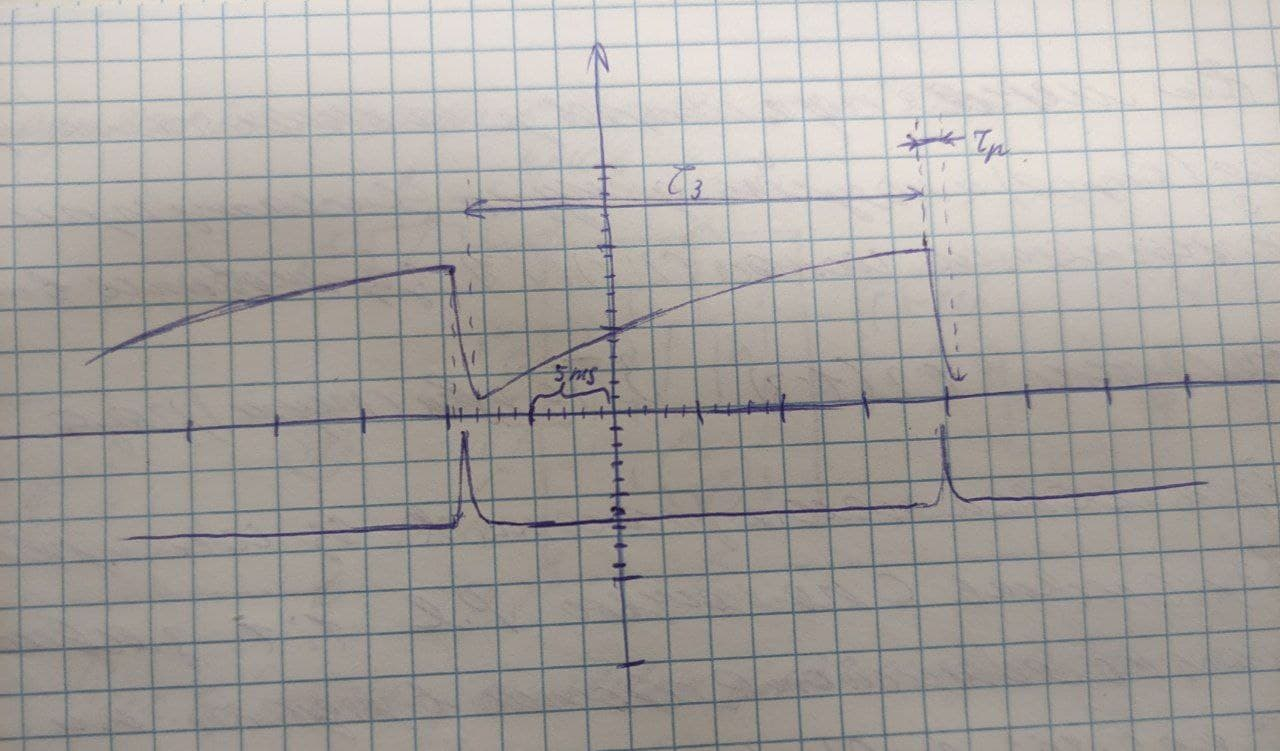
\includegraphics[scale=0.2]{photo1.jpg}
\caption{Пилообразная картинка}
\label{fig:Image1}
\end{figure}

\vspace{0.5cm}

Уменьшая сопротивление магазина определим $R_{\textit{кр}}$, при котором пропадают колебания. $R_{\textit{кр}} = 150$ \textit{кОм}, при этом теоретическое значение критического сопротивления $R_\textit{теор} = 15$ \textit{кОм}. Такие различия возникают в результате неидеальности схемы и возникновения в ней помех.

\vspace{0.5cm}

Подадим сигнал с генератора на вход \textit{Х} осциллографа. Меняя частоту ЗГ получим на экране фигуру Лиссажу без самопересечений. Не меняя параметров релаксационного генератора получим фигуры Лиссажу при соотношении частот 2:1, 3:1, 1:2, 1:3.

\begin{figure}[h!]
\centering
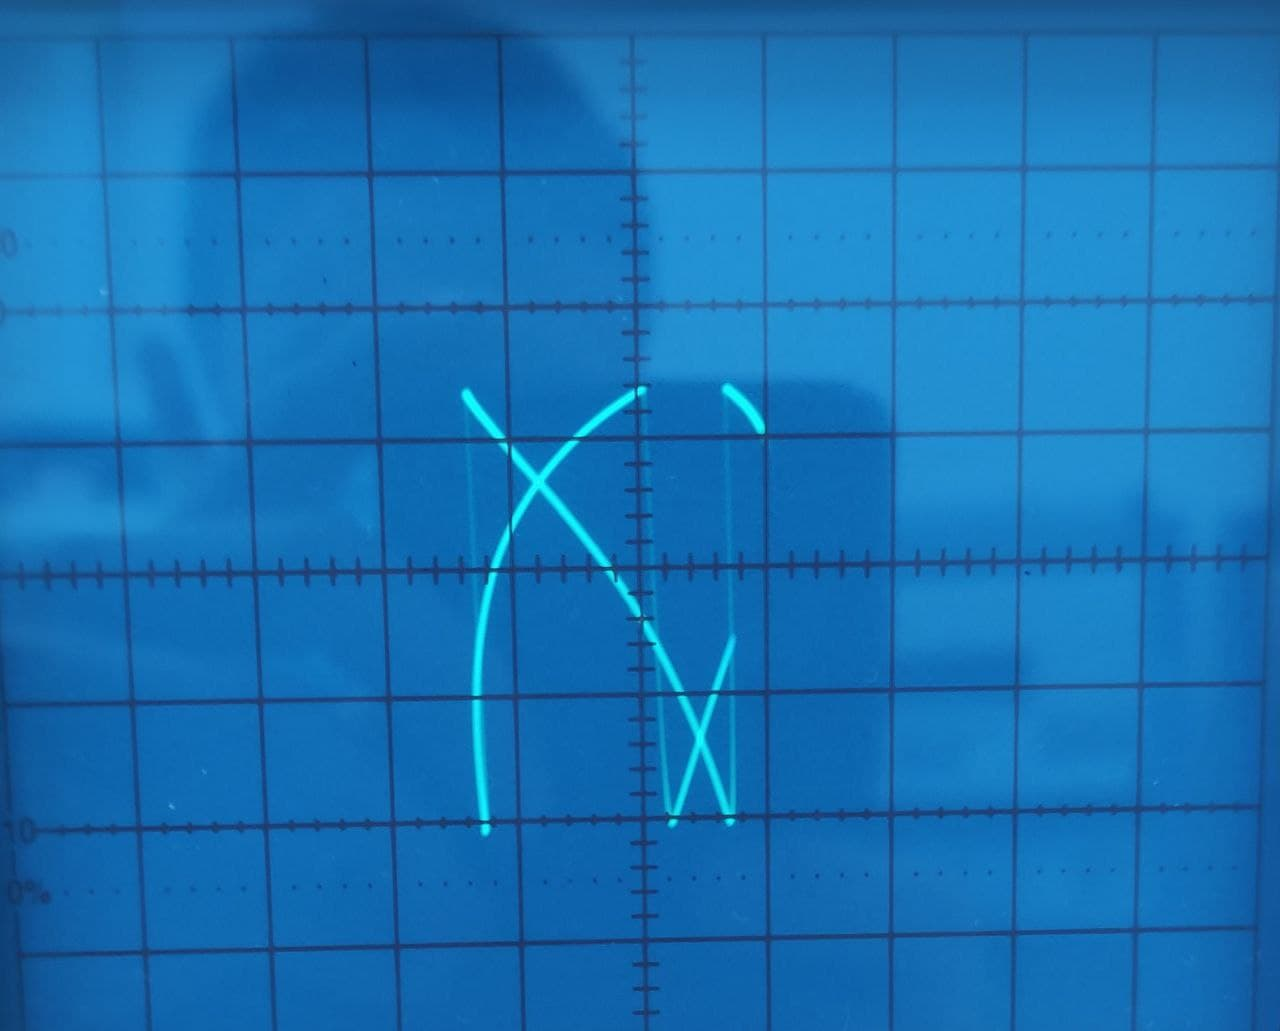
\includegraphics[scale=0.15]{31.jpg}
\caption{Соотношение частот 3:1}
\label{fig:Image1}
\end{figure}

\begin{figure}[h!]
\centering
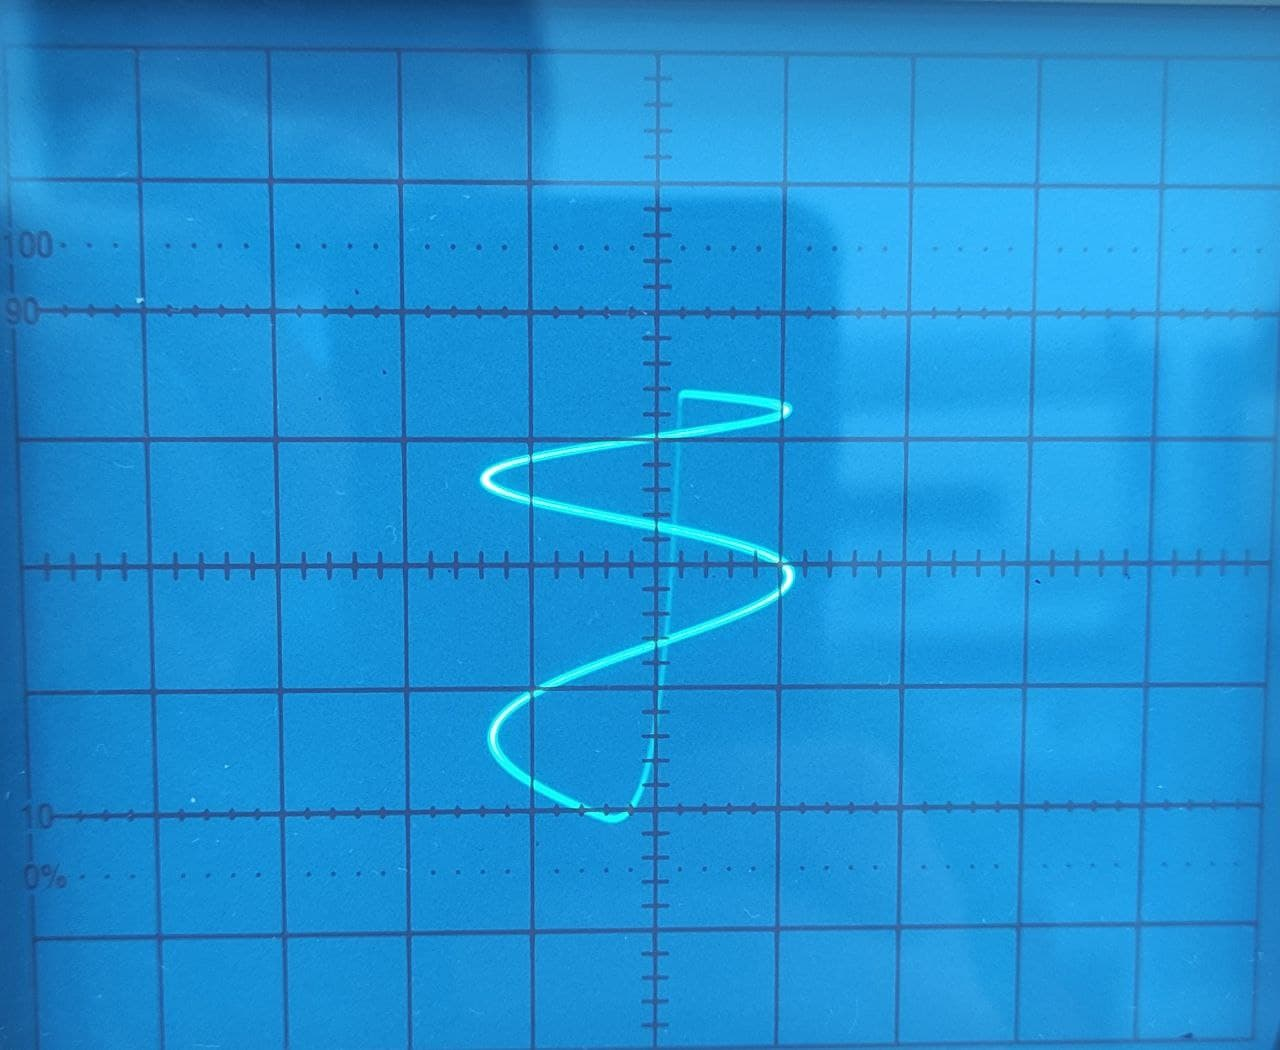
\includegraphics[scale=0.15]{12.jpg}
\caption{Соотношение частот 1:2}
\label{fig:Image1}
\end{figure}

\begin{figure}[h!]
\centering
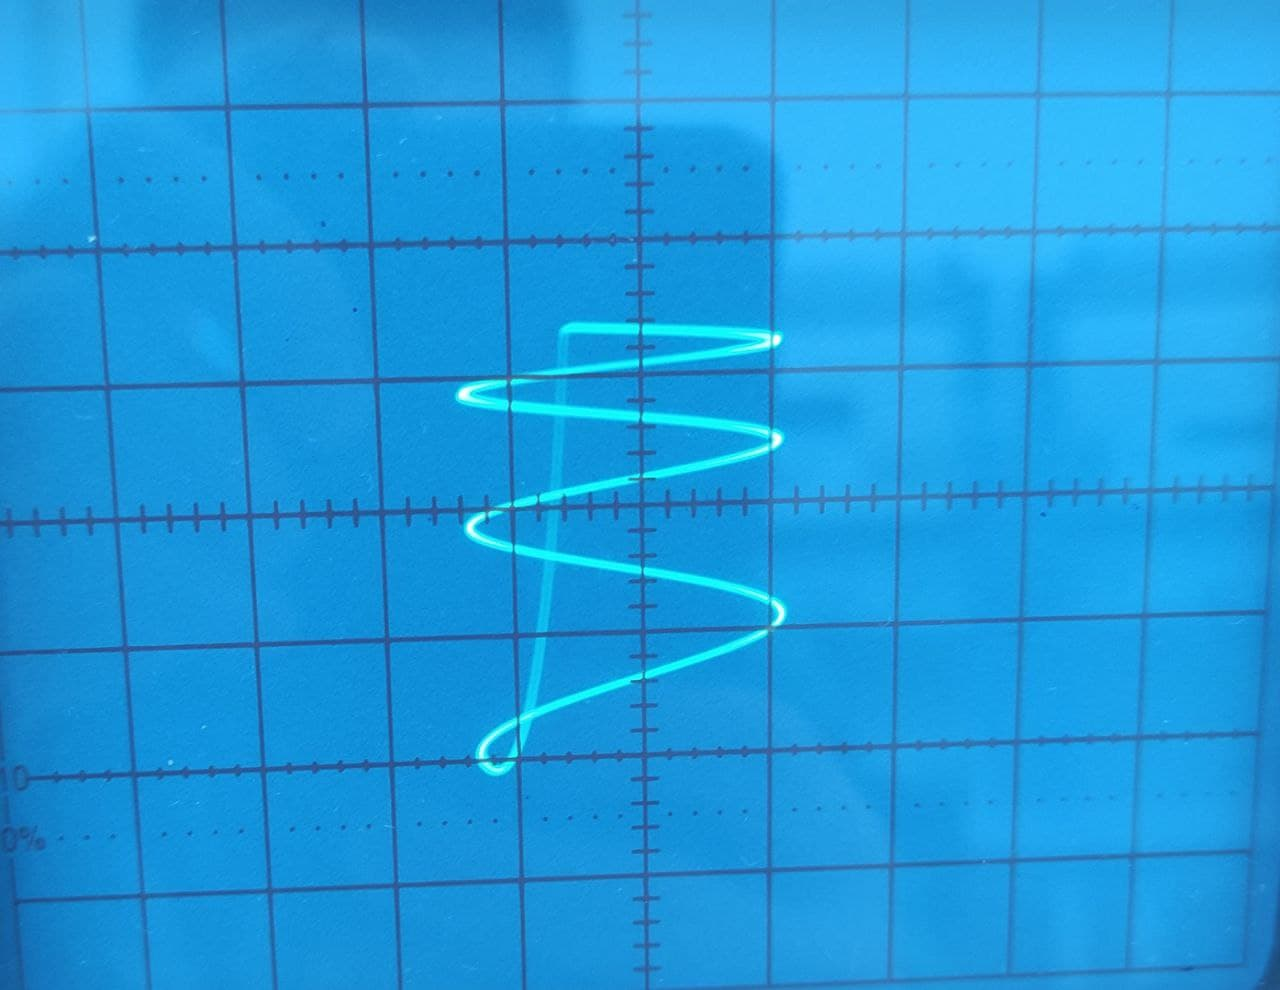
\includegraphics[scale=0.15]{13.jpg}
\caption{Соотношение частот 1:3}
\label{fig:Image1}
\end{figure}

\vspace{0.5cm}

\newpage

При значении сопротивления $R = 3R_{\textit{кр}}$ снимем с помощью фигур Лиссажу зависимость частоты колебаний от емкости \textit{С}.

\begin{figure}[h!]
\centering
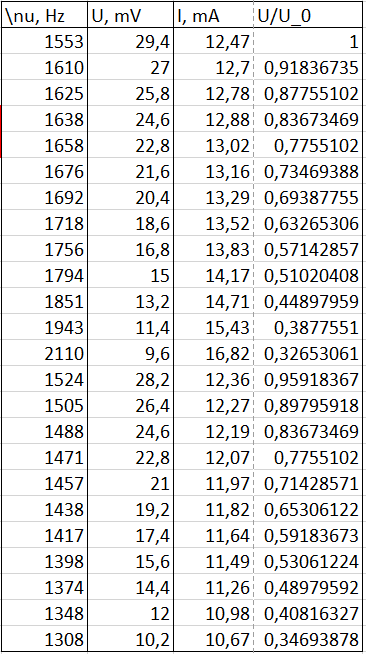
\includegraphics[scale=0.8]{table2.png}
\caption{Зависмость T(C)}
\label{fig:Image1}
\end{figure}

\vspace{0.5cm}
\newpage
Аналогично проведем серию измерений $\nu = f(R)$ при постоянной емкости $C = 5\cdot 10^{-2}$ \textit{мкФ}, меняя величину \textit{R} от максимального значения до критического.

\begin{figure}[h!]
\centering
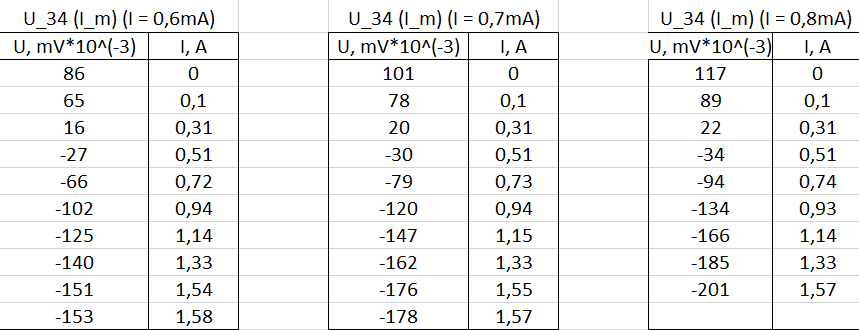
\includegraphics[scale=0.8]{table3.png}
\caption{Зависимость T(R)}
\label{fig:Image1}
\end{figure}

\vspace{0.5cm}

Построим графики по получившимся данным. Также рядом с ними построим графики теореических значений рассчитанных по формуле:

\begin{equation}
T = RC\ln \frac{U - V_2}{U - V_1},
\end{equation}

где $V_1$ и $V_2$ значения указанные в первой таблице.

\vspace{0.5cm}

\begin{figure}[h!]
\centering
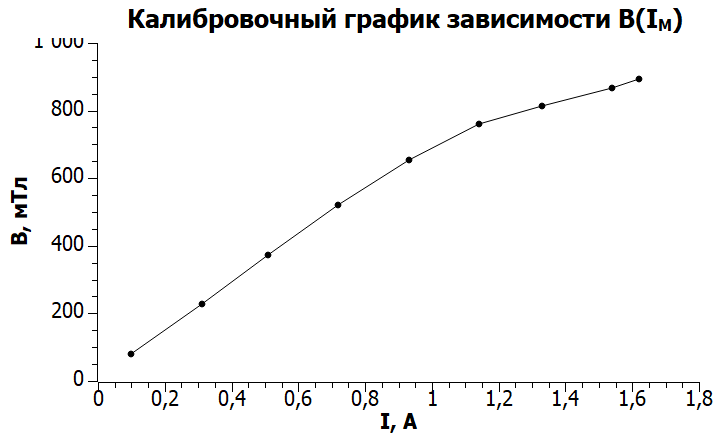
\includegraphics[scale=1]{Graph2.png}
\label{fig:Image1}
\end{figure}

\begin{figure}[h!]
\centering
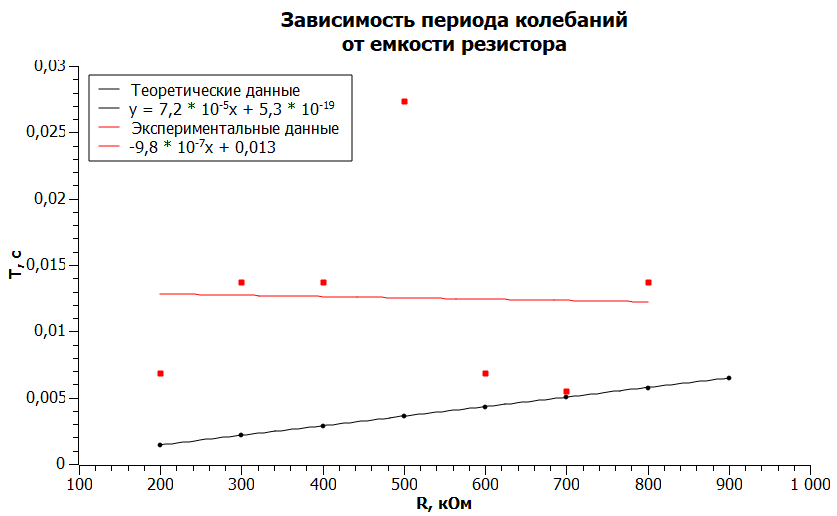
\includegraphics[scale=1]{Graph3.png}
\label{fig:Image1}
\end{figure}

\newpage

Можем заметить, что наклоны экспериментальной и теоретической прямой заметно отличаются. Это происходит в результате неидеальности собранной схемы и метода измерения частоты колебаний. Мы можем рассчитать динамический потенциал гашения для получившихся экспериментальных прямых по формуле:

\[T \approx RC \ln \frac{U - V_2}{U - V_1}\]

Тогда в случае зависимости $T(C)$ получим $V_2 = 85,34$ \textit{В}, а в случае зависимости $T(R)$ получим $V_2 = 86,39$ \textit{В}, что ожидаемо, так как у нашей прямой отрицательный наклон. Оценивать погрешности для данных величин нет смысла, так как мы имеем очень большой расброс точек на графике, следовательно проблема кроется и методе измерения.

\section*{Вывод}\

Познакомились с релаксационными колебаниями и стабилитроном. Получили плохие данные для зависимостей $T(C)$ и $T(R)$, так как пользовались плохим методом определения частоты колебаний. Также получили фигуры Лиссажу на осциллографе при помощи ЗГ.

\end{document}